\documentclass[10pt]{article}

\usepackage{enumerate}
\usepackage{amsmath}
\usepackage{amssymb}
\usepackage{amsthm}
\usepackage{array}
\usepackage[all]{xy}
\usepackage{fancyhdr}
\usepackage{euscript}
\usepackage{graphics}
\usepackage{cancel}
\usepackage{fancybox}
\usepackage{tikz}
\usepackage{tikz-3dplot}
\usepackage{pgf}
\usepackage{pgfplots}
\usepackage[all]{xy}
\usepackage{graphicx}
\pgfplotsset{compat=1.14}

\usepackage{pstricks}
\usepackage{pst-plot}

\usepackage{setspace}
\onehalfspacing

\setlength{\oddsidemargin}{.5in}
\setlength{\evensidemargin}{.5in}
\setlength{\textwidth}{6.in}
\setlength{\topmargin}{0in}
\setlength{\headsep}{.20in}
\setlength{\textheight}{8.5in}


\pdfpagewidth 8.5in
 \pdfpageheight 11in


%General
\newcommand{\WW}{\mathbb {W}}
\newcommand{\ZZ}{\mathbb{Z}}
\newcommand{\RR}{\mathbb {R}}
\newcommand{\II}{\mathbb {I}}
\newcommand{\QQ}{\mathbb {Q}}
\newcommand{\CC}{\mathbf C}
\newcommand{\NN}{\mathbb {N}}
\newcommand{\Zn}[1]{\mathbf{Z}/#1\mathbf{Z}}
\newcommand{\Znx}[1]{(\mathbf{Z}/#1\mathbf{Z})^\times}
\newcommand{\X}{\times} 
\newcommand{\set}[2]{\left\{#1 : #2\right\}}          
\newcommand{\sett}[1]{\left\{#1\right\}}                
\newcommand{\nonempty}{\neq\varnothing}
\newcommand{\ds}{\displaystyle}
\newcommand{\abs}[1]{\left| {#1} \right|}
\newcommand{\qedbox}{\rule{2mm}{2mm}}
\renewcommand{\qedsymbol}{\qedbox}											
\newcommand{\aand}{\qquad\hbox{and}\qquad}
\newcommand{\e}{\varepsilon}
\newcommand{\tto}{\rightrightarrows}
\newcommand{\gs}{\geqslant}
\newcommand{\ls}{\leqslant}
\renewcommand{\tilde}{\widetilde}
\renewcommand{\hat}{\widehat}
\newcommand{\norm}[1]{\left\| #1 \right\|}
\newcommand{\md}[3]{#1\equiv#2\;(\mathrm{mod}\;#3)}     
\newcommand{\gen}[1]{\left\langle #1 \right\rangle}
\renewcommand{\Re}{\operatorname{Re}}
\renewcommand{\Im}{\operatorname{Im}}
\newcommand{\zero}{\boldsymbol{0}}

\newcommand{\be}[1]{\textbf{\emph{#1}}}
\newcommand{\hhat}[1]{\hat{\! \hat{#1}}}

\newcommand{\fto}[1]{\xrightarrow{\hspace{4pt} #1 \hspace{4pt}}}
\newcommand{\flto}[1]{\xrightarrow{\quad #1 \quad}}



\newcommand{\dist}{\operatorname{dist}}
\newcommand{\esssup}{\operatorname{ess\:sup}}
\newcommand{\id}{\operatorname{id}}
\newcommand{\card}{\operatorname{card}}

\newcommand{\dmu}{\:\mathrm{d}\mu}
\newcommand{\dm}{\:\mathrm{d}m}
\newcommand{\dx}{\:\mathrm{d}x}
\newcommand{\dt}{\:\mathrm{d}t}
\newcommand{\dz}{\:\mathrm{d}z}
\newcommand{\dtheta}{\:\mathrm{d}\theta}
\newcommand{\dw}{\:\mathrm{d}w}

%Algebra
\newcommand{\Sym}{\operatorname {Sym}}
\newcommand{\Stab}{\operatorname {Stab}}
\newcommand{\M}{\operatorname{M}}
\newcommand{\GL}{\operatorname{GL}}
\newcommand{\PGL}{\operatorname{PGL}}
\newcommand{\SL}{\operatorname{SL}}
\newcommand{\PSL}{\operatorname{PSL}}
\newcommand{\Heis}{\operatorname{Heis}}
\newcommand{\Aff}{\operatorname{Aff}}
\newcommand{\Aut}{\operatorname{Aut}}
\newcommand{\image}{\operatorname{im}}
\newcommand{\Syl}[2]{\operatorname{\emph{Syl}}_{#1}\left(#2\right)}
\newcommand{\Hom}{\operatorname{Hom}}
\newcommand{\Tor}{\operatorname{Tor}}
\newcommand{\Gal}{\operatorname{Gal}}
\newcommand{\ch}{\operatorname{ch}}
\newcommand{\rad}{\operatorname{rad}}
\newcommand{\iso}{\cong}
\newcommand{\normal}{\unlhd}
\newcommand{\semi}{\rtimes}
\newcommand{\Nm}{\operatorname {N}}
\newcommand{\Tr}{\operatorname {Tr}}
\newcommand{\disc}{\operatorname {disc}}








%Euler Script Characters
\newcommand{\esa}{\EuScript{A}}
\newcommand{\esb}{\EuScript{B}}
\newcommand{\esc}{\EuScript{C}}
\newcommand{\esd}{\EuScript{D}}
\newcommand{\ese}{\EuScript{E}}
\newcommand{\esf}{\EuScript{F}}
\newcommand{\esg}{\EuScript{G}}
\newcommand{\esh}{\EuScript{H}}
\newcommand{\esi}{\EuScript{I}}
\newcommand{\esj}{\EuScript{J}}
\newcommand{\esk}{\EuScript{K}}
\newcommand{\esl}{\EuScript{L}}
\newcommand{\esm}{\EuScript{M}}
\newcommand{\esn}{\EuScript{N}}
\newcommand{\eso}{\EuScript{O}}
\newcommand{\esp}{\EuScript{P}}
\newcommand{\esq}{\EuScript{Q}}
\newcommand{\esr}{\EuScript{R}}
\newcommand{\ess}{\EuScript{S}}
\newcommand{\est}{\EuScript{T}}
\newcommand{\esu}{\EuScript{U}}
\newcommand{\esv}{\EuScript{V}}
\newcommand{\esw}{\EuScript{W}}
\newcommand{\esx}{\EuScript{X}}
\newcommand{\esy}{\EuScript{Y}}
\newcommand{\esz}{\EuScript{Z}}

%Calligraphic Characters
\newcommand{\cala}{\mathcal{A}}
\newcommand{\calb}{\mathcal{B}}
\newcommand{\calc}{\mathcal{C}}
\newcommand{\cald}{\mathcal{D}}
\newcommand{\cale}{\mathcal{E}}
\newcommand{\calf}{\mathcal{F}}
\newcommand{\calg}{\mathcal{G}}
\newcommand{\calh}{\mathcal{H}}
\newcommand{\cali}{\mathcal{I}}
\newcommand{\calj}{\mathcal{J}}
\newcommand{\calk}{\mathcal{K}}
\newcommand{\call}{\mathcal{L}}
\newcommand{\calm}{\mathcal{M}}
\newcommand{\caln}{\mathcal{N}}
\newcommand{\calo}{\mathcal{O}}
\newcommand{\calp}{\mathcal{P}}
\newcommand{\calq}{\mathcal{Q}}
\newcommand{\calr}{\mathcal{R}}
\newcommand{\cals}{\mathcal{S}}
\newcommand{\calt}{\mathcal{T}}
\newcommand{\calu}{\mathcal{U}}
\newcommand{\calv}{\mathcal{V}}
\newcommand{\calw}{\mathcal{W}}
\newcommand{\calx}{\mathcal{X}}
\newcommand{\caly}{\mathcal{Y}}
\newcommand{\calz}{\mathcal{Z}}

%Gothic Characters
\newcommand{\fraka}{\mathfrak{a}}
\newcommand{\frakb}{\mathfrak{b}}
\newcommand{\frakc}{\mathfrak{c}}
\newcommand{\frakd}{\mathfrak{d}}
\newcommand{\frake}{\mathfrak{e}}
\newcommand{\frakf}{\mathfrak{f}}
\newcommand{\frakg}{\mathfrak{g}}
\newcommand{\frakh}{\mathfrak{h}}
\newcommand{\fraki}{\mathfrak{i}}
\newcommand{\frakj}{\mathfrak{j}}
\newcommand{\frakk}{\mathfrak{k}}
\newcommand{\frakl}{\mathfrak{l}}
\newcommand{\frakm}{\mathfrak{m}}
\newcommand{\frakn}{\mathfrak{n}}
\newcommand{\frako}{\mathfrak{o}}
\newcommand{\frakp}{\mathfrak{p}}
\newcommand{\frakq}{\mathfrak{q}}
\newcommand{\frakr}{\mathfrak{r}}
\newcommand{\fraks}{\mathfrak{s}}
\newcommand{\frakt}{\mathfrak{t}}
\newcommand{\fraku}{\mathfrak{u}}
\newcommand{\frakv}{\mathfrak{v}}
\newcommand{\frakw}{\mathfrak{w}}
\newcommand{\frakx}{\mathfrak{x}}
\newcommand{\fraky}{\mathfrak{y}}
\newcommand{\frakz}{\mathfrak{z}}

\newcommand{\frakA}{\mathfrak{A}}
\newcommand{\frakB}{\mathfrak{B}}
\newcommand{\frakC}{\mathfrak{C}}
\newcommand{\frakD}{\mathfrak{D}}
\newcommand{\frakE}{\mathfrak{E}}
\newcommand{\frakF}{\mathfrak{F}}
\newcommand{\frakG}{\mathfrak{G}}
\newcommand{\frakH}{\mathfrak{H}}
\newcommand{\frakI}{\mathfrak{I}}
\newcommand{\frakJ}{\mathfrak{J}}
\newcommand{\frakK}{\mathfrak{K}}
\newcommand{\frakL}{\mathfrak{L}}
\newcommand{\frakM}{\mathfrak{M}}
\newcommand{\frakN}{\mathfrak{N}}
\newcommand{\frakO}{\mathfrak{O}}
\newcommand{\frakP}{\mathfrak{P}}
\newcommand{\frakQ}{\mathfrak{Q}}
\newcommand{\frakR}{\mathfrak{R}}
\newcommand{\frakS}{\mathfrak{S}}
\newcommand{\frakT}{\mathfrak{T}}
\newcommand{\frakU}{\mathfrak{U}}
\newcommand{\frakV}{\mathfrak{V}}
\newcommand{\frakW}{\mathfrak{W}}
\newcommand{\frakX}{\mathfrak{X}}
\newcommand{\frakY}{\mathfrak{Y}}
\newcommand{\frakZ}{\mathfrak{Z}}

%Lowercase Bold Letters
\newcommand{\bfa}{\mathbf{a}}
\newcommand{\bfb}{\mathbf{b}}
\newcommand{\bfc}{\mathbf{c}}
\newcommand{\bfd}{\mathbf{d}}
\newcommand{\bfe}{\mathbf{e}}
\newcommand{\bff}{\mathbf{f}}
\newcommand{\bfg}{\mathbf{g}}
\newcommand{\bfh}{\mathbf{h}}
\newcommand{\bfi}{\mathbf{i}}
\newcommand{\bfj}{\mathbf{j}}
\newcommand{\bfk}{\mathbf{k}}
\newcommand{\bfl}{\mathbf{l}}
\newcommand{\bfm}{\mathbf{m}}
\newcommand{\bfn}{\mathbf{n}}
\newcommand{\bfo}{\mathbf{o}}
\newcommand{\bfp}{\mathbf{p}}
\newcommand{\bfq}{\mathbf{q}}
\newcommand{\bfr}{\mathbf{r}}
\newcommand{\bfs}{\mathbf{s}}
\newcommand{\bft}{\mathbf{t}}
\newcommand{\bfu}{\mathbf{u}}
\newcommand{\bfv}{\mathbf{v}}
\newcommand{\bfw}{\mathbf{w}}
\newcommand{\bfx}{\mathbf{x}}
\newcommand{\bfy}{\mathbf{y}}
\newcommand{\bfz}{\mathbf{z}}




%Customized Theorem Environments
\newtheoremstyle%
{custom}%
{}%                         Space above
{}%													Space below
{}%													Body font
{}%                         Indent amount
{}%                         Theorem head font
{.}%                        Punctuation after heading
{ }%                        Space after heading
{\thmname{}%                Additional specifications for theorem head
\thmnumber{}%
\thmnote{\bfseries #3}}%

\newtheoremstyle%
{Theorem}%
{}%
{}%
{\itshape}%
{}%
{}%
{.}%
{ }%
{\thmname{\bfseries #1}%
\thmnumber{\;\bfseries #2}%
\thmnote{\;(\bfseries #3)}}%

%Theorem Environments
\theoremstyle{Theorem}
\newtheorem{theorem}{Theorem}[section]
\newtheorem{cor}{Corollary}[section]
\newtheorem{lemma}{Lemma}[section]
\newtheorem{prop}{Proposition}[section]
\newtheorem*{nonumthm}{Theorem}
\newtheorem*{nonumprop}{Proposition}
\theoremstyle{definition}
\newtheorem{definition}{Definition}[section]
\newtheorem*{answer}{Answer}
\newtheorem*{solution}{Solution}
\newtheorem*{nonumdfn}{Definition}
\newtheorem*{nonumex}{Example}
\newtheorem{ex}{Example}[section]
\theoremstyle{remark}
\newtheorem{remark}{Remark}[section]
\newtheorem*{note}{Note}
\newtheorem*{notation}{Notation}
\theoremstyle{custom}
\newtheorem*{cust}{Definition}
\fancypagestyle{firststyle}
{
   \fancyhead[L]{\textbf{Name:}}
   \fancyhead[R]{\textbf{Worksheet 3: Tangent Lines, Limit Def-Derivative, Deriv on Graph}}
   \fancyfoot[R]{ Thomas Luckner } %{\footnotesize Page \thepage\ of \pageref{LastPage}}
}






\begin{document}
\thispagestyle{firststyle}
\pagestyle{plain}

Thoughts:\\\\
We talked about this shortly one time, but it is best to go in a little more depth for you guys since many instructors forget to even say what a tangent line is. Let's start with that.
\begin{definition}[Tangent line at $a$]
A line, say $L$, is tangent to a curve at $a$ if it touches the curve LOCALLY at $a$ only. 
\end{definition}
\noindent The confusing word is locally. Here what we mean by locally is we only used $a$ to find this line $L$. No other point was used. This is different from a secant line which is the line connecting two points.\\
Now we got the definition out of the way. So, what is it in a mathematic sense? How do I find $L$? Well a line is of the form: $mx+b$ where $m$ is the slope and $b$ is the $y$-intercept. 
We need to find these things to get our line! remeber once we have our slope and a point we can use point slope form ($y-y_1=m(x-x_1)$) to find the $y$-intercept. Thus, finding the slope is our focus.  This is no obvious task. What we do notice is that if we take two points and find the secant line between those two, we can find the slope of that! What if I take the point I care about for my tangent line and keep moving the other point closer and closer? Eventually I would get the same point I want! This is the idea for finding the slope of the tangent line. When I say closer and closer this should remind you of something you have been doing... LIMITS! Let's see how this works algorithmically.\\
Say we want the tangent line at $x$. Let's take any point $h$ away from $x$ and find the slope of the secant line. 
\[
\dfrac{f(x+h)-f(x)}{x+h-x}=\dfrac{f(x+h)-f(x)}{h}.
\]
Now we want this point $x+h$ to be as close as possible to $x$. That means we want $h$ as small as possible! LIMITS!
\[
m_t=\lim_{h\rightarrow 0}\dfrac{f(x+h)-f(x)}{h}.
\]
There it is! We can reframe this as $a$ our tangent line point and $b$ the other $x$ value and get
\[
m_t=\lim_{b\rightarrow a}\dfrac{f(b)-f(a)}{b-a}.
\]
Now here is the fun part. We have the slop of the tangent line. This mathematical object is very important!
\begin{definition}[Derivative at $x$]
Let $f'(a)$ be the derivative at $a$ defined by
\[
f'(a)=\lim_{h\rightarrow 0}\dfrac{f(a+h)-f(a)}{h}
\]
or
\[
f'(a)=\lim_{b\rightarrow a}\dfrac{f(b)-f(a)}{b-a}.
\]
\end{definition}
\noindent In other words, the slope of the tangent line IS the derivative at $a$! Replace $a$ with $x$ and now it is a function! We also call the derivative the \textbf{instantaneous rate of change}. This just means the rate of change but only at a point instead of an average of two points.
\newpage
\noindent Graphically: This is harder to explain without seeing a picture. \\\\
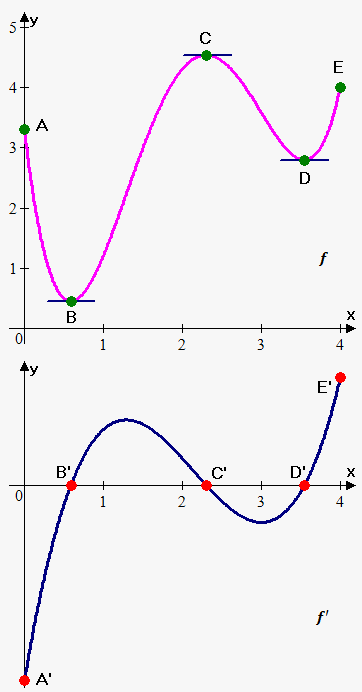
\includegraphics[width=4cm]{deriv.png}\\
The top is the function and the bottom is its derivative. Any point for which the slope is 0 is a zero for the derivative. In other words, slope at $a$ 0 $\Rightarrow f'(a)=0$. Always mark these first! Then look to the left and right of these 0's. Is the slope positive or negative? If negative $f'<0$. If positive $f'>0$. This is how you sketch the graph of the derivative from the function.\\
To go from graph of derivative to function, notice how your peaks and troughs are the points of slope 0. This means any 0's of the derivative are peaks and troughs! Plot those first. Then see if the derivative is positive or negative to the left and right. Let;s consider to the left for now. If the derivative is above the $x$-axis, then the slope is positive and we draw a positive slope like C in the picture! If below the $x-axis$, then the slope is negative and we draw a negative slope like B in the picture.
\newpage
Problems:
\begin{enumerate}[1.]
\item Find the equation of the tangent line for the given curve and point.
\begin{enumerate}[a.]
\item $y=x^3-3x+1$, (2,3)
\begin{solution}
\begin{align*}
m_t&=\ds\lim_{h\rightarrow 0}\dfrac{(x+h)^3-3(x+h)+1-(x^3-3x+1)}{h}=\ds\lim_{h\rightarrow 0}\dfrac{h(x^2+2x^2+2xh+xh+h^2-3)}{h}\\[2pt]
&=\ds\lim_{h\rightarrow 0} x^2+2x^2+2xh+xh+h^2-3\\[2pt]
&=3x^2-3.
\end{align*}
$\Rightarrow m_t(2)=3(2)^2-3=9.$\\\\
Now we have a point and the slope so we can use point-slope form!
\[
y-3=9(x-2) \Rightarrow y=9x-15.
\]
\end{solution}
\item $y=\dfrac{2x+1}{x+2}$, (1,1)
\begin{solution}
\begin{align*}
m_t&=\lim_{h\rightarrow 0}\dfrac{\dfrac{2(x+h)+1}{x+h+2}-\dfrac{2x+1}{x+2}}{h}\\[2pt]
&=\lim_{h\rightarrow 0} \dfrac{\dfrac{(2x+2h+1)(x+2)-(2x+1)(x+h+2)}{(x+h+2)(x+2)}}{h}\\[2pt]
&=\lim_{h\rightarrow 0}\dfrac{\left(\dfrac{3h}{(x+h+2)(x+2)}\right)}{h}\\[2pt]
&= \lim_{h\rightarrow 0} \dfrac{3}{(x+h+2)(x+2)}\\[2pt]
&=\dfrac{3}{(x+2)^2}.
\end{align*}
$\Rightarrow m_t(1)=\dfrac{3}{1+2)^2}=\dfrac{1}{3}.$\\\\
Point-slope form.
\[
y-1=\dfrac{1}{3}(x-1) \Rightarrow y=\dfrac{1}{3}x+\dfrac{2}{3}.
\]
\end{solution}
\end{enumerate}
\newpage
\item Each limit is the derivative of a function at a value. Determine the original function.
\begin{enumerate}[a.] 
\item $\ds\lim_{h\rightarrow 0}\dfrac{(1+h)^{10}-1}{h}$
\begin{solution}
Notice our $x$ is 1 from the $1+h$. The power 10 is seen also here $(1^{10}=1)$. Thus, $f(x)=x^{10}$ and $x=1$.
\end{solution}
\item $\ds\lim_{h\rightarrow 0}\dfrac{\cos(\pi+h)+1}{h}$
\begin{solution}
Here we notice we have $\pi+h$ inside the cosine. Thus, $x=\pi$ and $f(x)=\cos(x)$ since $\cos(\pi)=-1$.
\end{solution}
\item $\ds\lim_{t\rightarrow 1}\dfrac{t^4+t-2}{t-1}$
\begin{solution}
This form is not our $h$ form! Here we have $a\rightarrow b$. Thus, $t=1$ here and $f(t)=t^4+t$.
\end{solution}

\end{enumerate}
\item Find $f'(a)$. In other words, no limit if possible!
\begin{enumerate}[a.]
\item $f(x)=\dfrac{4}{\sqrt{1-x}}$
\begin{solution}
\begin{align*}
f'(a)&=\lim_{h\rightarrow 0}\dfrac{\dfrac{4}{\sqrt{1-a-h}}-\dfrac{4}{\sqrt{1-a}}}{h}\\[2pt]
&=\lim_{h\rightarrow 0}\dfrac{\dfrac{4\sqrt{1-a}-4\sqrt{1-a-h}}{\sqrt{(1-a-h)(1-a)}}}{h}\\[2pt]
&=\lim_{h\rightarrow 0} \dfrac{4\dfrac{(\sqrt{1-a}-\sqrt{1-a-h})(\sqrt{1-a}+\sqrt{1-a-h})}{\sqrt{(1-a-h)(1-a)}(\sqrt{1-a}+\sqrt{1-a-h})}}{h}\\[2pt]
&=\lim_{h\rightarrow 0}\dfrac{4\dfrac{h}{\sqrt{(1-a-h)(1-a)}(\sqrt{1-a}+\sqrt{1-a-h})}}{h}\\[2pt]
&=\lim_{h\rightarrow 0}\dfrac{4}{\sqrt{(1-a-h)(1-a)}(\sqrt{1-a}+\sqrt{1-a-h})}\\[2pt]
&=\dfrac{4}{(1-a)(2\sqrt{1-a})}=\dfrac{2}{(1-a)^{3/2}}.
\end{align*}
\end{solution}
\newpage
\item $f(x)=\dfrac{2t+1}{t+3}$
\begin{solution}
\begin{align*}
f'(a)&=\lim_{h\rightarrow 0}\dfrac{\dfrac{2(a+h)+1}{a+h+3}-\dfrac{2a+1}{a+3}}{h}\\[2pt]
&=\lim_{h\rightarrow 0}\dfrac{\dfrac{(2a+2h+1)(a+3)-(2a+1)(a+h+3)}{(a+h+3)(a+3)}}{h}\\[2pt]
&=\lim_{h\rightarrow 0} \dfrac{\dfrac{5h}{(a+h+3)(a+3)}}{h}\\[2pt]
&=\lim_{h\rightarrow 0}\dfrac{5}{(a+h+3)(a+3)}\\[2pt]
&=\dfrac{5}{(a+3)^2}
\end{align*}
\end{solution}
\item $f(x)=3x^2-4x+1$
\begin{solution}
\begin{align*}
f'(a)&=\lim_{h\rightarrow 0}\dfrac{3(a+h)^2-4(a+h)+1-(3a^2-4a+1)}{h}\\[2pt]
&=\lim_{h\rightarrow 0} \dfrac{h(6a+3h-4)}{h}\\[2pt]
&=\lim_{h\rightarrow 0} 6a-4.
\end{align*}
\end{solution}
\end{enumerate}
\newpage
\item Sketch the graph of the derivative of the function below. 
\begin{solution}
The derivative is 0 at A C and E. Positive from A to C and E to infinity. Negative from negative infinity to A and C to E.
\end{solution}
\begin{center}
\begin{tikzpicture}
	\draw (.83756544,-.07334178) node[label=below:{E}] {\textbullet};
	\draw (.26959444,.1295146672) node[label={C}] {\textbullet};
	\draw (-1.10716,-2.056172885) node[label={A}] {\textbullet};
	\draw (.5773502692,.0217947136) node[label={D}] {\textbullet};
	\draw (-.5773502692,-1.132905825) node[label={B}] {\textbullet};
	\draw[step=.5cm,gray,very thin] (-4,-4) grid (4,4);
      \draw[thick,<->] (-4,0) -- (4,0) node[right] {$x$};
      \draw[thick,<->] (0,-4) -- (0,4) node[above] {$y$};
      \draw[very thick, scale=1,domain=-1.6:1.66,smooth,variable=\x,blue] plot ({\x},{\x*\x*\x*\x-2*\x*\x+\x});
     
    \end{tikzpicture}
    \end{center}
\item Assume the above is the derivative. Sketch the graph of the function.
\begin{solution}
A, B, C, D, E are all useless in this! 0 is a minimum or trough. Between D and E is a maximum. Another minimum after E. If the deriviative graph continued in the negative direction, there would be a maximum before A. Now Connect the dots.
\end{solution}
\end{enumerate}
\end{document}







